\documentclass[a4paper,10pt]{scrartcl}

\usepackage[utf8]{inputenc}
\usepackage[ngerman]{babel}
\usepackage[T1]{fontenc}
\usepackage{amsmath}
\usepackage[section]{placeins}
\usepackage{graphicx}
\usepackage{esvect}
\usepackage{amssymb}



\title{Praktikum B Vorbereitung zu Versuch "of"}
\author{Leon Machtl und Raphael Lehner}
\date{12.12.2019}

\begin{document}
	\maketitle
	\tableofcontents
	\newpage
	
	\section{Einleitung zum Versuch}
Ziel des Versuchs ``Optisches Filtern'' ist es, die Grundzüge der Abbeschen Abbildungstheorie näher zu bringen. Theoretische Grundlage liefern dabei die Konzepte der Geometrischen Optik, die Abbildungseigenschaften von Linsen und insbesondere die Bildkonstruktion durch Strahlenoptik, welche aus dem Versuch ``Optische Geräte'' bekannt sind, sowie die Kenntnisse zur Beugung und Interferenz sowie Kohärenz von Licht. Voraussetzung für den Vorgang des optischen Filterns ist Planung eines realisierbaren, geeigneten Aufbaus von Lichtquelle und Linsen. Durch gezielte Eingriffe in den optischen Aufbau soll der Beugung des Lichts für die Theorie der optischen Abbildung sowie für den Bau von optischen Instrumenten anschaulich vermittelt werden, um die dabei auftretenden Auflösungsgrenzen zu verstehen.\\
	Die geometrische Optik vermittelt kein Konzept, die Leistungsfähigkeit optischer Systeme abzuschätzen. Tatsächlich glaubten auch die Mikroskophersteller bis zu den Arbeiten von Abbe in der Mitte des 19. Jahrhunderts, dass die einzige Begrenzung des räumlichen Auflösungsvermögens durch die technischen Fähigkeiten der Linsenhersteller gegeben war. Auf Basis der Wellenoptik wissen wir heute aber, dass die grundlegende Längenskala für die Auflösungsgrenze optischer Systeme die Wellenlänge des verwendeten Lichts ist. (Die Vorhersagen der geometrischen Optik und der Wellenoptik sind äquivalent zu den Aussagen der klassischen Physik und der Quantenmechanik. Während in der klassischen Physik prinzipiell keinerlei Grenzen für die Messgenauigkeit existieren, hat man in der Quantenmechanik aufgrund der Heisenberg'schen Unschärferelation eine Grenze vorgegeben.)\\
	Mithilfe der folgenden Vorbereitungsfragen und -aufgaben soll der Versuchsaufbau geplant werden. Ziel ist es, diesen Aufbau während des Praktikums anhand dieser Planung aufzubauen und zu justieren. Dazu stehen folgende Komponenten zur Verfügung:\\
  	\begin{itemize}  
  		\item Optische Bank
  		\item Stativ
  		\item HeNe-Laser
  		\item bikonvexe Linsen, jeweils eine Linse der Brennweite:
  			\begin{itemize}
  				\item $f = \SI{5}{mm}$
  				\item $f = \SI{50}{mm}$
  				\item $f = \SI{100}{mm}$
  				\item $f = \SI{200}{mm}$
  			\end{itemize}
  		\item Optische Liniengitter
  		\item Optische Kreuzgitter
  		\item diverse Blenden (verstellbarer Spalt, Irisblenden)
  		\item 1 Strahlenteiler
  		\item Oberflächenspiegel
  		\item Beobachtungsschirm
  	\end{itemize}
	
	\section{Fragen zur Vorbereitung und Durchführung}
		
		\subsection{Frage 1}
			Wie lautet die Abbildungsgleichung für Linsen und was bedeuten die einzelnen Größen?\\
			\\
			Die Abbildungsgleichung für Linsen lautet 
			\begin{align*}
			\frac{1}{f}=\frac{1}{g}+\frac{1}{b}
			\end{align*}
			Dabei steht \(f\) für die Brennweite der Linse (Abstand des Brennpunkts von der Hauptebene), \(g\) für die Gegenstandsweite (Abstand des Gegenstands von der Hauptebene) und \(b\) für die Bildweite (Abstand des Bildes von der Hauptebene).\\
			Für den Abbildungsmaßstab \(A\) gilt die Beziehung
			\begin{align*}
			A=\frac{y'}{y}
			\end{align*}
			wobei \(y\) die Gegenstandsgröße und \(y'\) die Bildgröße bezeichnet. Zudem gilt außerdem
			\begin{align*}
			A=\frac{b}{g}
			\end{align*}
			Und somit folgt aus den beiden Beziehungen für \(A\)
			\begin{align*}
			\frac{y'}{y}=\frac{b}{g}
			\end{align*}
			
		\subsection{Frage 2}
			Graphische Darstellung der Größen der Abbildungsgleichung und Konstruktion des Gegenstands \(G\). Vergleich der konstruierten Werte für Bildgröße und Bildweite mit den berechneten.\\
			\\
			\begin{figure}[h]
\centering
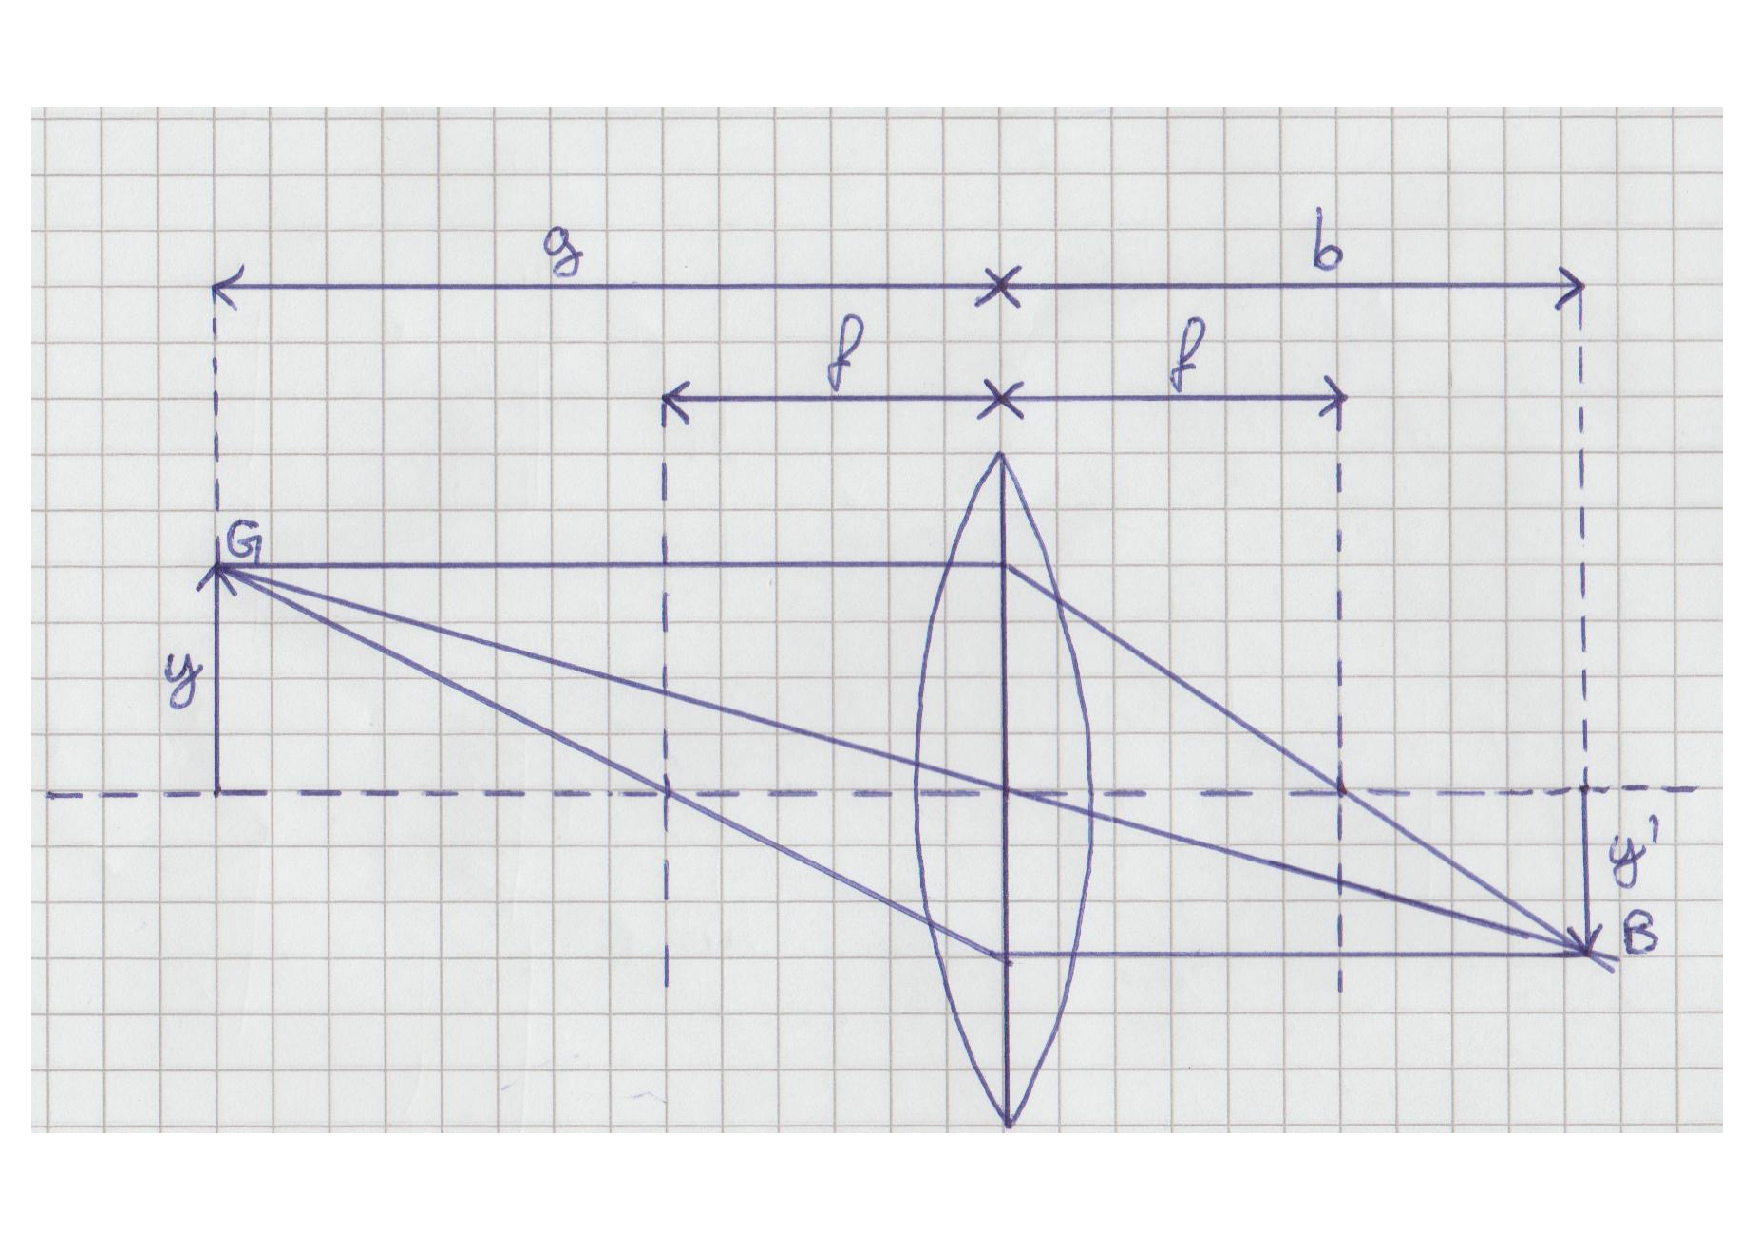
\includegraphics[width=0.9\textwidth]{./Bilder/ofa2}

\end{figure}
\FloatBarrier
			\\
			In Skizze abgemessene Werte:\\
			\(f=\SI{30}{mm}, g=\SI{70}{mm}, b=\SI{52}{mm},y=\SI{20}{mm},y'=\SI{15}{mm}\) \\
			Umstellen der Abbildungsgleichung aus Aufgabe 1:
			\begin{align*}
			b=\frac{1}{\frac{1}{f}-\frac{1}{g}}=\SI{52,5}{mm}
			\end{align*}
			\begin{align*}
			y'=y\frac{b}{g}=\SI{30}{mm}\frac{\SI{52,5}{mm}}{\SI{70}{mm}}=\SI{15}{mm}
			\end{align*}
			Die berechneten Werte stimmen also sehr gut mit den gemessenen Werten überein.
			
		\subsection{Frage 3}
			Im Versuch benutzt man einen Laserstrahl, dessen enges Ausgangsstrahlbündel näherungsweise zu einem breiteren Parallelstrahl aufgeweitet wird.\\
			Dafür sollen zwei Linsen \(L_{1}\) und \(L_{2}\) verwendet werden. Dabei gilt für die Brennweite von \(L_{1}\) \(f_{1}=5mm\), wobei die  Aufweitung 10-fach sein soll. Für die Linse \(L_{2}\) stehen Linsen mit einer Brennweite von \(50mm\),\(100mm\) oder \(200mm\) zur Verfügung. Welche davon sollte man wählen? Wie groß müssen die Linsendurchmesser mindestens sein?\\
			\\
			Eine Aufweitung kann mit verschiedenen Linsensystemen erreicht werden, beispielsweise mit umgekehrten Teleskop-Aufbauten. Eine Möglichkeit wäre eine umgekehrte Kepler-Anordnung, diese besteht aus zwei bikonvexen Linsen mit einem gemeinsamen Brennpunkt. Dieser Aufbau kann für die Aufweitung eines Hochleistungs-Lasers jedoch nachteilig sein, da es in diesem gemeinsamen Brennpunkt zu einer sehr hohen Leistungsdichte kommen kann, die zur Funkenentladung der aufgeheizten Luft führen kann. Besser ist es daher, eine umgekehrte Galilei-Anordnung zu verwenden. Diese besteht aus einer bikonvexen und einer bikonkaven Linse. Zwar gibt es auch hier einen gemeinsamen Brennpunkt, dieser ist jedoch nicht reell. 
			Somit wird der Nachteil der Kepler-Anordnung umgangen. Der in diesem versuch verwendete Laser ist aber schwach genug, um die Kepler-Anordnung verwenden zu können.\\
			\\
						\begin{figure}[h]
\centering
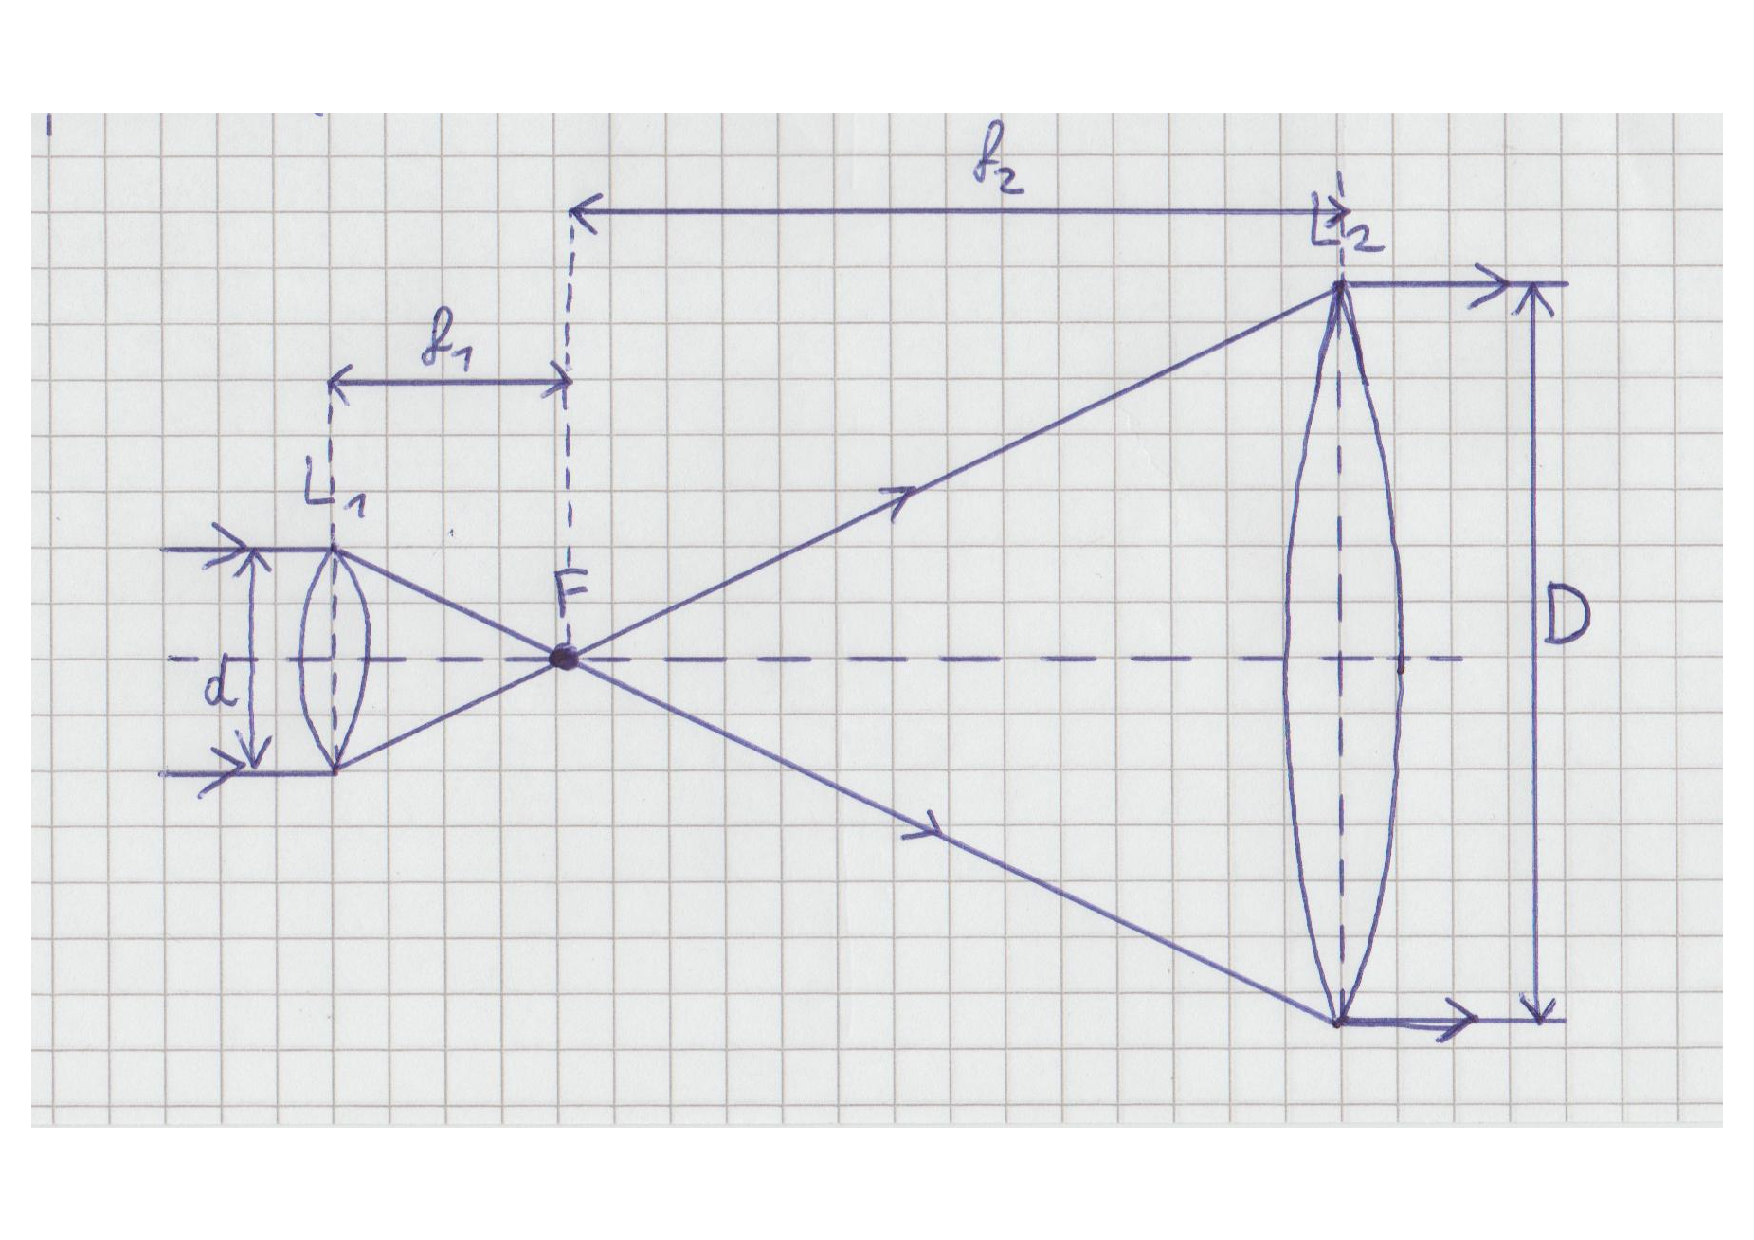
\includegraphics[width=0.9\textwidth]{./Bilder/ofa3}

\end{figure}
\FloatBarrier
			\\
			Für eine 10-fach Aufweitung gilt \(A=10\). Mit einer Linse \(L_{1}\) mit \(f_{1}=5mm\) gilt dann:
			\begin{align*}
			A=\frac{D}{d}=\frac{f_{2}}{f_{1}}
			\end{align*}
			was im Versuch zu optische Geräte gezeigt wurde. Durch Umformung erhält man
			\begin{align*}
			f_{2}=Af_{1}=10 \cdot 5mm=50mm
			\end{align*}
			Man sollte also für \(L_{2}\) die Linse mit der Brennweite von \(50mm\) verwenden, um eine 10-fache Aufweitung zu erreichen. Bei optischen Abbildungen an Linsen tritt immer Beugung auf, ein Punkt wird also nicht auf genau einen Punkt abgebildet, sondern auf ein sogenanntes Beugungsscheibchen oder auch Airy-Scheibchen abgebildet. Der Radius dieses Beugungsscheibchens beträgt dabei ungefähr
			\begin{align*}
			r=1,22\frac{\lambda f}{d}
			\end{align*}
			wobei \(\lambda\) die Wellenlänge des einfallenden Lichtes, \(f\) die Brennweite der Linse und \(d\) der Durchmesser der Linse ist. Damit das Beugungsscheibchen möglichst klein bleibt, muss also der Durchmesser von \(L_{1}\) groß sein im Vergleich zum Durchmesser des Laserstrahls sein. Seine mindeste Größe muss der Breite des Strahls entsprechen. Der Durchmesser von \(L_{2}\) muss dann für die gewünschte Vergrößerung 10-mal so groß sein, wie der von \(L_{1}\).
			
		\subsection{Frage 4}
			Erläutern Sie die Begriffe „Primäres Bild“ und „Sekundäres Bild“ der Abbeschen Abbildungstheorie.
			Wo liegen diese Bilder? Wie kann man das primäre Bild mathematisch beschreiben?\\
			\\
			Wird ein Objekt in einen mikroskopartigen Aufbau, wie der umgekehrten Kepler-Anordnung, gebracht, so entsteht in der Brennebene von \(L_{1}\) ein für die Topologie des betrachteten Objektes charakteristisches Interferenzmuster. Dieses Interferenzmuster wird nach Ernst Abbe als primäres Bild bezeichnet. Das sekundäre Bild bezeichnet dann die Vereinigung des primären Bildes (also des Interferenzmusters) mit den vom Objekt geradlinig ausgehenden Strahlen, die von dem optischen Instrument abgebildet werden. Dabei handelt es sich um ein entweder vergrößertes oder verkleinertes Bild des betrachteten Objektes. Dieses Bild befindet sich in der Bildebene. Das strukturierte Bild des Objektes ergibt sich erst durch diese Vereinigung der geradlinigen Strahlen mit dem Interferenzmuster, das durch Beugung entsteht.\\
			\\
			Wie ensteht das Interferenzmuster?\\
			\\
			Das Problem wird hier vereinfacht anhand der Beugung an einem Spalt betrachtet, obwohl in der Realität Beugungsphänomene an jeder Struktur eines Objektes auftreten. Passieren Lichtstrahlen einen Spalt, so entstehen dahinter kugelförmige Wellen, die sich in alle Richtungen ausbreiten. Dies kann man vereinfacht als zwei verschiedene Strahlensets betrachten. Ein Strahl ändert nach dem Durchgang durch den Spalt seine Richtung nicht (Strahl 0. Ordnung), die anderen werden alle um einen gewissen Winkel \(\beta\) abgelenkt. Tritt nun der Fall ein, dass \(\beta\) von einer solchen Größe ist, dass der Gangunterschied von einem Strahl, der von einem Ende des Spalts ausgeht, im Vergleich zu dem Strahl, der von der anderen Seite des Spalts ausgeht, \(\Delta=n\lambda\) beträgt, so existiert zu jedem Lichtstrahl exakt ein interferenzfähiger Partner, der eine Phasenverschiebung von \(\frac{\lambda}{2}\) besitzt. Die beiden Partner interferieren also destruktiv und löschen sich somit vollständig aus. Nun gibt es auch \(beta\) bei denen der Gangunterschied genau \(\Delta=(n+0,5)\lambda\) beträgt. In einem solchen Fall interferieren die Strahlenpartner konstruktiv miteinander, werden also verstärkt. Somit ergibt sich das Interferenzmuster für die verschiedenen \(\beta\). In der Realität handelt es sich natürlich um Kugelwellen und keine Strahlen, die Erklärung durch die Strahlen ist jedoch an dieser stelle ausreichend.\\
			\\
			Die Strahlen 0. Ordnung werden gemäß der bekannten Weise der geometrischen Optik gebrochen, übertragen jedoch keine Informationen über die sogenannte "Textur" des abzubildenden Objekts. Nutzt man eine sehr enge Blende so, dass nur die Strahlen 0. Ordnung passieren können, so kann man das Objekt in der Abbildung nicht erkennen. Ein erkennbares Abbild ensteht erst durch die Überlagerung der Strahlen 0. Ordnung mit dem Interferenzmuster (primäres Bild). Das Bild wird genauer und schärfer, je mehr Strahlen höherer Ordnung 
			(größeren \(\beta\)) abgebildet werden, daher hängt die Linsengröße direkt mit der Qualität des Bildes zusammen.
			
			\subsection{Frage 5}
		Das abzubildende Objekt sei nun ein Liniengitter. Das Gitter wird mit kohärentem Licht beleuchtet. Die Gitterspalte stehen dabei senkrecht auf der Zeichenebene. Konstruiere primäres sowie sekundäres Bild und skizziere den Intensitätsverlauf (qualitativ) in den entsprechenden Ebenen. Berücksichtige bei der Konstruktion die Beugungsmaxima 0. Sowie 1. Ordnung.
					
					\begin{figure}[h]
\centering
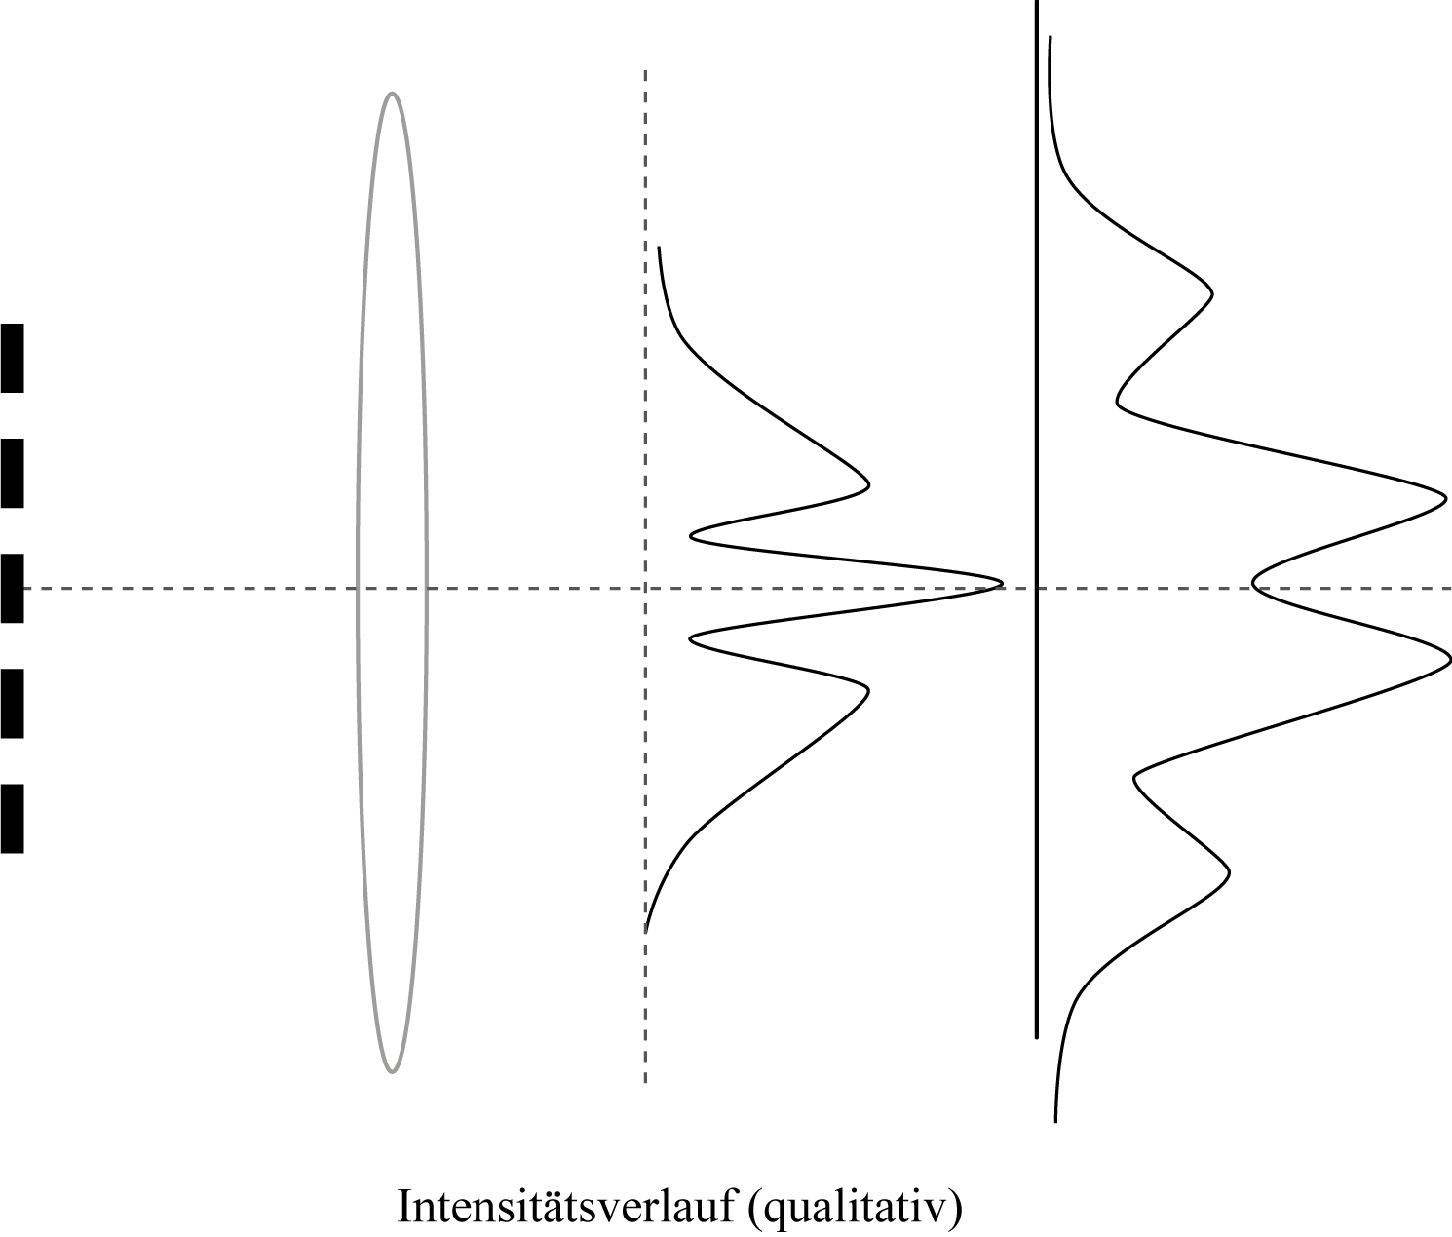
\includegraphics[width=0.9\textwidth]{./Bilder/ofa52}

\end{figure}					
					\begin{figure}[h]
\centering
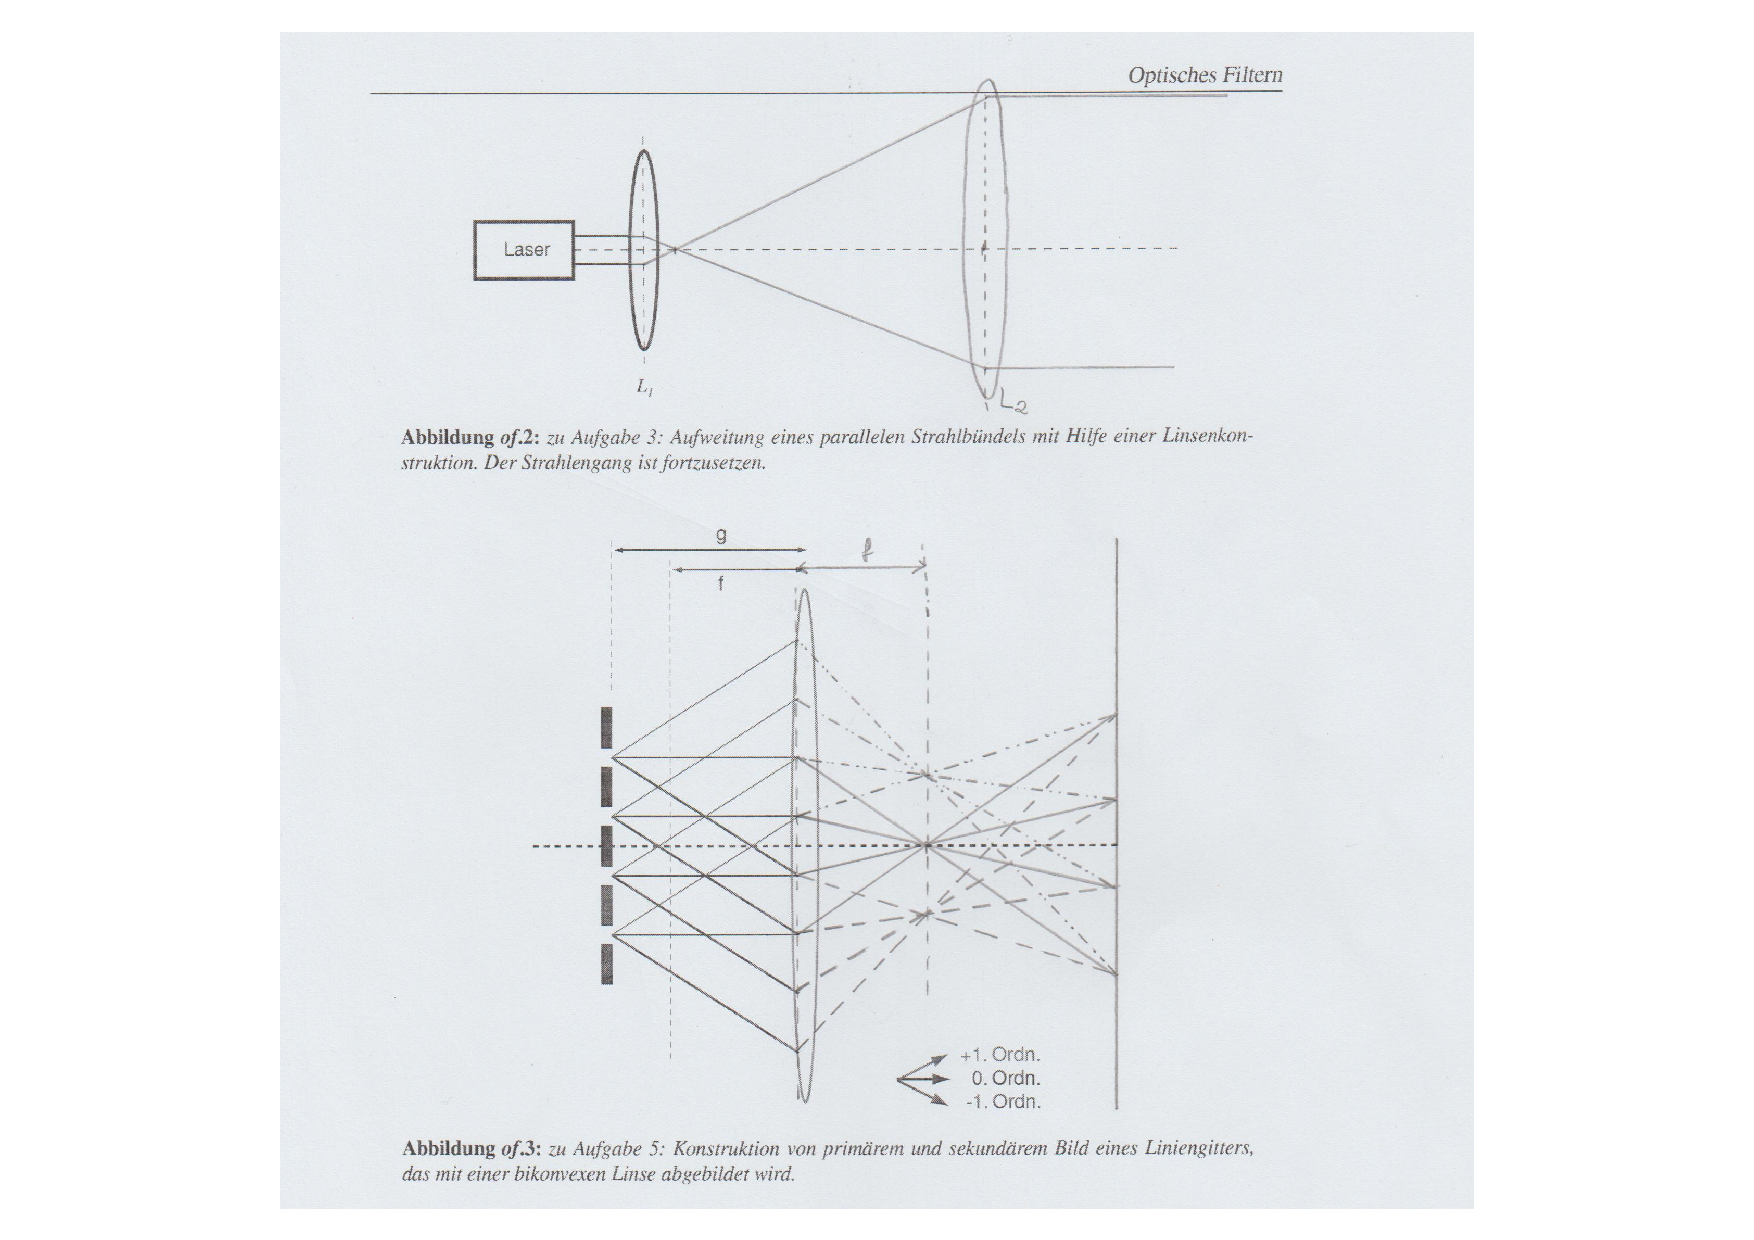
\includegraphics[width=0.9\textwidth]{./Bilder/ofa5}

\end{figure}
\FloatBarrier
		\\
		\\
	\subsection{Frage 6}
		Berechne den Abstand $\Delta x$ benachbarter Punkte in der hinteren Brennebene von\\Aufgabe Nr. 5.
		\\
		\\
		Die Lage der Beugungsmaxima eines Gitters ist gegeben durch:
			\[\sin(\Psi_{m,max}) = \frac{\lambda}{d} \cdot m\]
		\begin{tabular}{ll}
			$m$ & Beugungsordnung\\
			$\sin(\Psi_{m,max})$ & Beugungswinkel des $m$-ten Beugungsmaximums\\
			$\lambda$ & Wellenlänge des beleuchtenden Lichtes\\
			$d$ & Abstand der Gitterlinien
		\end{tabular}
		\\
		\\
		Für $m = 1$ gilt: $\sin(\Psi_{1,max}) = \frac{\lambda}{d} \approx \tan(\Psi_{1,max}) = \frac{\Delta x}{f}$ (Kleinwinkelnäherung).\\
		Mithilfe dieser Näherung folgt:
			\[\Delta x \approx \frac{\lambda}{d} \cdot f\]
		An diesen Punkten interferieren die Lichtstrahlen konstruktiv. Es entstehen dort Intensitätsmaxima.

	\subsection{Frage 7}
		Um die Auswirkungen von Eingriffen am primären Bild auf das Endbild beobachten zu können, ist es hilfreich, das Endbild (sekundäres Bild) mit dem primären Bild zu vergleichen. Dies geschieht am bequemsten, wenn beide Bilder vergrößert nebeneinander auf dem Beobachtungsschirm dargestellt werden. Die Problemstellung besteht darin, zwei Bilder, die sich an unterschiedlichen Positionen im Strahlengang befinden, in einer Beobachtungsebene (Beobachtungsschirm) abzubilden.\\
		Dies kann mit untenstehendem Aufbau (nicht maßstabsgetreu, alle Maße in mm) erreicht werden. Beschrifte den Aufbau vollständig und berechne die Brennweiten $f_1, f_2, f_4, f_5$ sowie die Abstände $a_1, a_2, a_3$ und $a_4 + a_5$. Berücksichtige bei der Wahl der Linsen die Liste der zur Verfügung stehenden Komponenten.
		\\
		\\
		Strahlenaufweitung (siehe Aufgabe 3): $f_1 = \SI{5}{mm}$ und $f_2 = \SI{50}{mm}$\\
		Daraus folgt: $a_1 = f_1 + f_2 = \SI{55}{mm}$\\
		Mit $f_3 = \SI{200}{mm}$ folgt $a_2 = f_3 = \SI{200}{mm}$
		Mit der Linsenformel ergibt sich:
			\[\frac{1}{f_4} = \frac{1}{\SI{200}{mm}} = \frac{1}{\SI{450}{mm}} + \frac{1}{a_3 + \SI{140}{mm}} \Rightarrow a_3 = \SI{220}{mm}\]
			\[\frac{1}{f_5} = \frac{1}{\SI{100}{mm}} = \frac{1}{\SI{110}{mm}} + \frac{1}{a_4 + a_5} \Rightarrow a_4 + a_5 = \SI{1100}{mm}\]
					\begin{figure}[h]
\centering
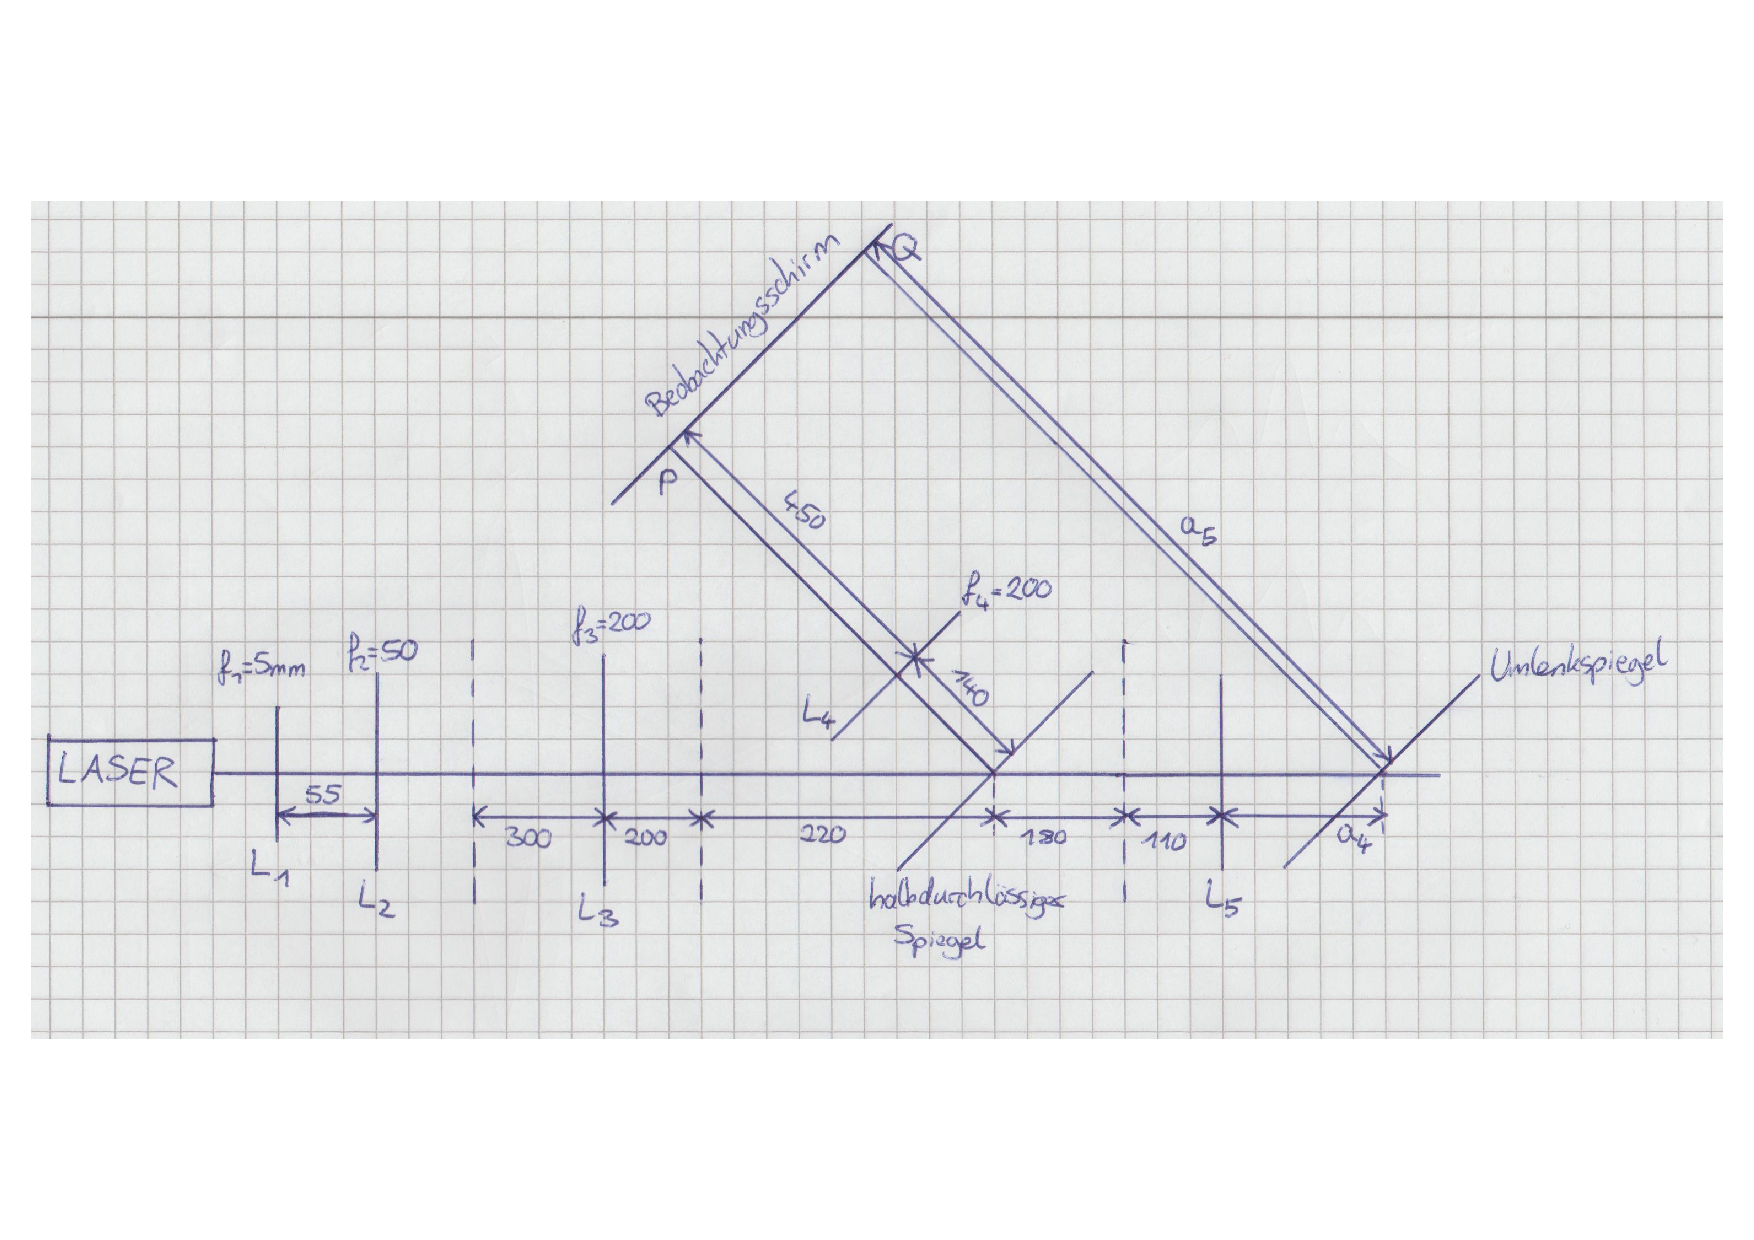
\includegraphics[width=0.9\textwidth]{./Bilder/ofa7}

\end{figure}
\FloatBarrier
		\\
	
	\subsection{Frage 8}
		Beschreiben Sie den Charakter der Bilder an den Orten P und Q am Leuchtschirm!
		\\
		\\
		\textbf{Punkt P.} Hier ist das primäre Bild sichtbar. Das Interferenzabbild wird scharf auf den Beobachtungsschirm abgebildet.\\
		\textbf{Punkt Q.} Hier ist das sekundäre Bild, also der Treffpunkt der Strahlen nullter Ordnung mit Strahlen höherer Ordnungen, sichtbar.
	\subsection{Frage 9}
		Überlegen Sie sich, wie Sie eine „optische Bank“ (also einen Aufbau mit mehreren optischen Komponenten wie z.B. Linsen) justieren sollten. Verdeutlichen Sie sich die Bedeutung einer optimalen Ausrichtung der optischen Komponenten auf der optischen Achse anhand (Abb. of.5). Setzen Sie den Strahlengang des parallel versetzt einfallenden Stahlbündels fort.Was beobachten Sie ?
		\\
		\\
		Lichstrahlen werden in einer Linse gebrochen und aufgeweitet. Werden die Linsenmitten nicht präzise auf der optischen Achse positioniert, trifft der Strahl mit einem entsprechend noch größeren Versatz zur Linsenachse auf die nächste Linse. Die Maxima der ersten Ordnung tragen somit nach einer Beugung am Gitter nicht mehr zum Bild bei, da die Apertur und damit der Durchmesser der nächsten Linse nach dem Gitter zu gering ist und gerade noch das Beugungsmaximum nullter Ordunng vom einfallenden Strahlenbündel erfassen kann. Die Intensität des Bildes am Schirm schließlich nimmt ab, im schlimmsten Fall ist es überhaupt nicht mehr zu sehen.
		\\
				\begin{figure}[h]
\centering
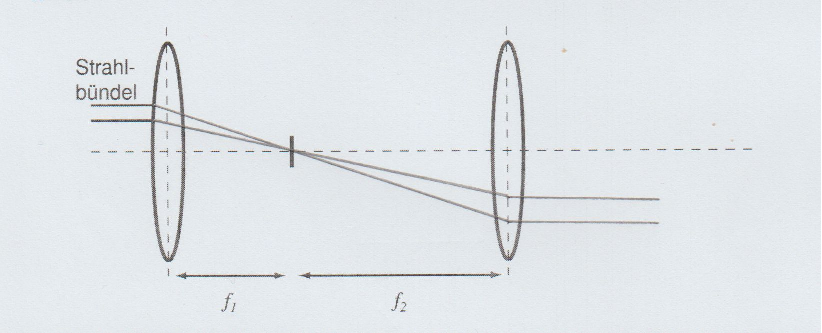
\includegraphics[width=0.9\textwidth]{./Bilder/ofa9}

\end{figure}
\FloatBarrier
			
\end{document}
